\documentclass[11pt]{article}

\usepackage[margin=1in]{geometry}
\usepackage{amsmath,amsfonts,amssymb}
\usepackage[none]{hyphenat}
\usepackage{fancyhdr}

\usepackage{multicol}
\usepackage{graphicx}
\usepackage{pgfplots}
\usepackage{wrapfig}

\pagestyle{fancy}
\fancyhead{}
\fancyfoot{}
\fancyhead[L]{\slshape \MakeUppercase{1.1 - Four Ways to Represent a Function}}
\fancyhead[R]{\slshape Ho Ngoc Van}
\fancyfoot[C]{\thepage}
\renewcommand{\footrulewidth}{0pt}

\newcommand{\soln}{\subsection*}
\newcommand{\qn}{\textit}

\begin{document}
	
\section*{Problem 1}

\qn{If $f(x)=x+\sqrt{2-x}$ and $g(x)=u+\sqrt{2-u}$, is it true that $f=g$?}

\soln{Solution}

True


\section*{Problem 2}

\qn{If $$f(x)=\frac{x^2-x}{x-1} \quad\mathrm{and}\quad g(x)=x$$ is it true that $f=g$?}

\soln{Solution}

False

\section*{Problem 3}

\qn{The graph of a function $g$ is given:}

\begin{figure}[h]
	\centering
	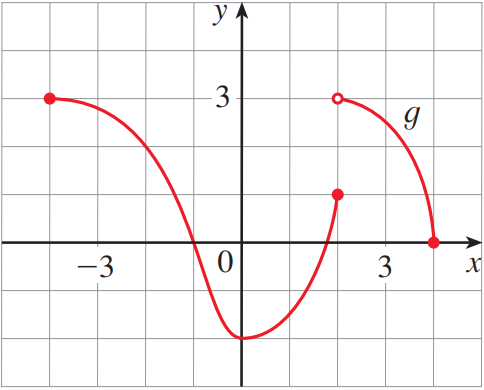
\includegraphics[width=0.3\linewidth]{figs/1.1.3}
\end{figure}

\begin{enumerate}
	\item \qn{State the values of $g(-2)$, $g(0)$, $g(2)$ and $g(3)$}
	\soln{Solution}
	$g(-2)=2 \quad g(0)=-2 \quad g(2)=1 \quad g(3)=2.5$
	
	\item \qn{For what value(s) of $x$ is $g(x)=3$?}
	\soln{Solution}
	$g(x)=3 \Rightarrow x=-4$
	
	\item \qn{For what value(s) of $x$ is $g(x) \leq 3$?}
	\soln{Solution}
	$g(x) \leq 3 \Rightarrow x \in [-4,4]$
	
	\item \qn{State the domain and range of $g$}
	\soln{Solution}
	$\mathrm{Domain}:[-4,4] \qquad\mathrm{Range}:[-2,3]$
	
	\item \qn{On what interval(s) is $g$ increasing?}
	\soln{Solution}
	$[0,2]$
\end{enumerate}

\section*{Problem 4}

\qn{The graph of $f$ and $g$ are given:}

\begin{figure}[h]
	\centering
	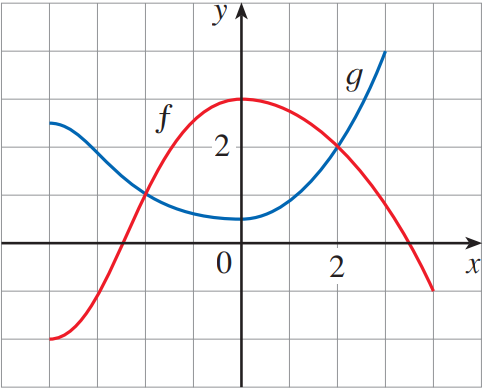
\includegraphics[width=0.3\linewidth]{figs/1.1.4}
\end{figure}

\begin{enumerate}
	\item \qn{State the values of $f(-4)$ and $g(3)$}
	\soln{Solution}
	$f(-4)=-2 \quad g(3)=4$
	
	\item \qn{Which is larger, $f(-3)$ or $g(-3)$?}
	\soln{Solution}
	$g(-3)$
	
	\item \qn{For what values of $x$ is $f(x)=g(x)$?}
	\soln{Solution}
	$x= \pm 2$
	
	\item \qn{On what interval(s) is $f(x) \leq g(x)$?}
	\soln{Solution}
	$[-4,-2] \cup [2,3]$
	
	\item \qn{State the solution of the equation $f(x)=-1$}
	\soln{Solution}
	$f(x)=-1 \Rightarrow x=-3$
	
	\item \qn{On what interval(s) is $g$ decreasing?}
	\soln{Solution}
	$[-4,0]$
	
	\item \qn{State the domain and range of $f$}
	\soln{Solution}
	$\mathrm{Domain}:[-4,4] \qquad\mathrm{Range}:[-2,3]$
	
	\item \qn{State the domain and range of $g$}
	\soln{Solution}
	$\mathrm{Domain}:[-4,3] \qquad\mathrm{Range}:[0.5,4]$
\end{enumerate}

\section*{Problem 5}

\qn{Figure 1 was recorded by an instrument operated by the California Department of Mines and Geology at the University Hospital of the University of Southern California in Los Angeles. Use it to estimate the range of the vertical ground acceleration function at USC during the North-ridge earthquake.}

\soln{Solution}

\section*{Problem 6}

\qn{In this section we discussed examples of ordinary, everyday functions: population is a function of time, postage cost is a function of package weight, water temperature is a function of time. Give three other examples of function from everyday life that are described verbally. What can you say about the domain and range of each of your functions? If possible, sketch a rough graph of each function.}

\soln{Solution}

\end{document}
